\textnormal{
The user has to open the file GUI.py. It can be done in command prompt using the command GUI.py. A new window opens which has a blank canvas and a few options on the right. The user has to draw a directed graph. The user can specify what he wants to draw. If there is a path, the button BDA* button is now clickable. These are the properties of the user interface: }
\begin{itemize}
    \item The user has an option to draw of the following: Vertex, Edge, Source Vertex, Goal Vertex. An edge can be drawn by clicking a vertex and dragging th pointer to other vertex. A vertex can be drawn by just clicking on the canvas. 
    \item Additionally, the user can edit an edge, update it's weights, delete a vertex or an edge. The graph is now made. 
    \item If there is no path from Source to Goal, an error window pops up that there is no path. The user can also clear the graph drawn and generate a randomized graph. 
    \item When the graph is connected from S to G, it checks for the heuristics. If it is not admissive, it prompts the user about it. However, the user can still choose to run BDA* as it is a logical error and the algorithm can still find a path. 
    \item At each iteration, the program will prompt one step and highlight the vertexes that are connected. The nodes reached from source are magenta in color and those from the goal are green in color. 
    \item Whenever the path is found, it prompts Done! and highlights the path.\
    \item The following are errors shown while running the program:
    \begin{itemize}
        \item An edge has to be from one vertex to another. It can't be random. 
        \item A source and goal vertex has to be specified. 
    \end{itemize}
\end{itemize}

\begin{figure}[h]
     \centering
     \begin{subfigure}{}
        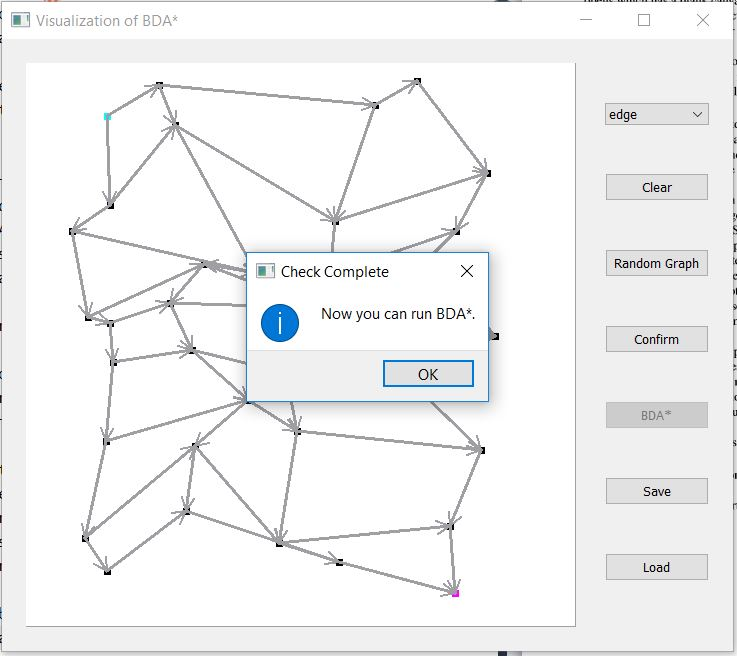
\includegraphics[width=0.4\textwidth]{Capture1.PNG}
        \caption{BDA* UI}
        \label{fig:1}
     \end{subfigure}
     \begin{subfigure}{}
        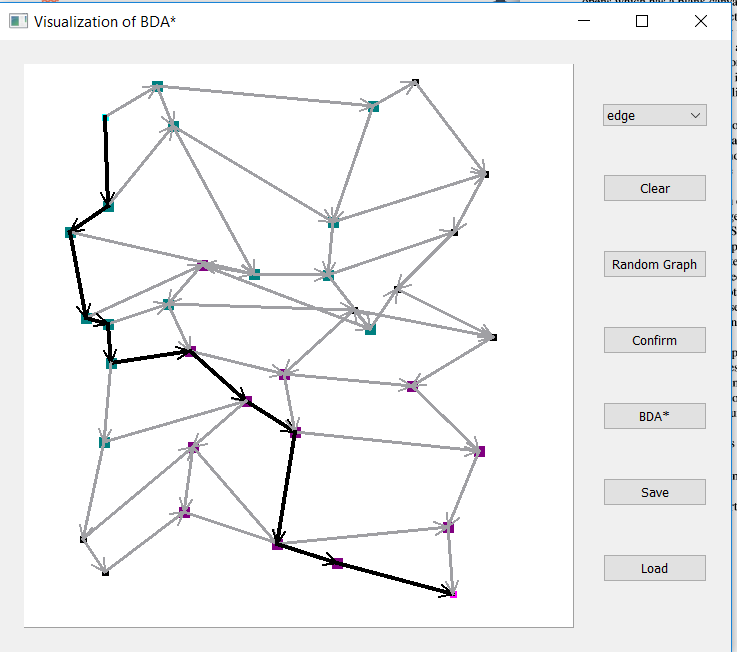
\includegraphics[width=0.4\textwidth]{Capture2.PNG}
        \caption{Showing Path}
        \label{fig:1}
        \end{subfigure}
     \end{figure}
